%\documentclass[11pt,professionalfonts,hyperref={pdftex,pdfpagemode=none,pdfstartview=FitH}]{beamer}
%\usepackage{times}
\documentclass[11pt,professionalfonts]{beamer}
\usefonttheme{serif}

\usepackage{presentation_packages}
\bibliography{library} % must be in the preamble when using biblatex package

\newcommand{\hilight}[1]{\colorbox{green}{#1}}

\definecolor{mygray}{gray}{0.9}
\definecolor{RoyalBlue}{rgb}{0.25,0.41,0.88}
\def\Emph{\textcolor{RoyalBlue}}

\definecolor{tmp}{rgb}{0.804,0.941,1.0}
\setbeamercolor{numerical}{fg=black,bg=tmp}
\setbeamercolor{exact}{fg=black,bg=red}

\mode<presentation> 
{
  \usetheme{Warsaw}
  \usefonttheme{serif}
  \setbeamercovered{transparent}
}

\setbeamertemplate{footline}%{split theme}
{%
  \leavevmode%
  \hbox{\begin{beamercolorbox}[wd=.5\paperwidth,ht=2.5ex,dp=1.125ex,leftskip=.3cm,rightskip=.3cm plus1fill]{author in head/foot}%
    \usebeamerfont{author in head/foot}\insertshorttitle
  \end{beamercolorbox}%
  \begin{beamercolorbox}[wd=.5\paperwidth,ht=2.5ex,dp=1.125ex,leftskip=.3cm,rightskip=.3cm]{title in head/foot}
%    \usebeamerfont{title in head/foot}\mypaper\hfill \insertframenumber/\inserttotalframenumber
    \usebeamerfont{title in head/foot}\hfill \insertframenumber/\inserttotalframenumber
  \end{beamercolorbox}}%
  \vskip0pt%
} \setbeamercolor{box}{fg=black,bg=yellow}


\title[Research Summary]{\large\bf  Professor Chrikjian Visit}

\author{Shankar Kulumani}

%\institute{\footnotesize
%{\normalsize Shankar Kulumani}\vspace*{0.2cm}\\
%  Flight Dynamics and Control Lab \\ 
%  Dept. of Mechanical and Aerospace Engineering\\ 
%  The George Washington University \\
%  Washington, DC\\ \vspace{10pt}
%  June 4, 2014 \\ \vspace{10pt}
%  }
\date{29 September 2016}

\institute{
\large{\textbf{Flight Dynamics \& Control Lab}}\\
  \begin{figure} %figure%
        
\includegraphics[width=0.75\textwidth]{gw_txh_2cs_pos}
    \end{figure}
}


\begin{document}
%=======================================================%

\setcounter{framenumber}{-1}
\begin{frame} %-----------------------------%
  \titlepage
\end{frame}   %-----------------------------%

\section{Orbital transfers using Reachability}
\subsection{Motivation}




\section{Constrained Attitude Control}
\subsection{Motivation}

\begin{frame} %--------------------------------%
	\frametitle{Motivation}
	\begin{itemize}
		\item Constrained rigid body attitude control
		\begin{itemize}
			\item Examples: spacecraft and robotic vehicles
			\item Attitude constraints: exposure concerns for optical payloads
			\begin{itemize}
				\item Bright objects: Sun, Moon
				\item Incoming debris
				\item Hostile action: directed energy
			\end{itemize}
		\end{itemize}
	\pause
	\item Previous approaches have several issues
	\begin{itemize}
		\item Attitude parameterizations: singularities/ambiguities
		\item Ad-hoc geometric approach: find intermediate points
		\item Randomized methods: stochastic stability result
		\item Barrier function: Motion planning/Optimal Control
	\end{itemize}
\end{itemize}
\end{frame} %----------------------------------%

\begin{frame}{Attitude Parameterizations}
	\begin{itemize}
		\item Euler Angles
		\begin{itemize}
			\item Minimal representation used for small attitude changes.
			\item Singularities exist for large angle slews: requires switching between 24 sequences
			\item Complicated trigonometric functions
		\end{itemize}
		\pause
		\item Quaternion 
		\begin{itemize}
			\item No singularities
			\item Two anti-podal quaternions for the same attitude
			\item Unwinding behavior 
		\end{itemize}
		\pause
		\item Geometric control
		\begin{itemize}
			\item Globally and uniquely characterize attitude: \( R \in \SO \)
			\item Singular representation of attitude 
			\item Geometrically exact
		\end{itemize}
	\end{itemize}
	
\end{frame}

\subsection{Research}

\begin{frame}{Research Objectives}
\begin{itemize}
	\item Attitude manuevers with state inequality constraints
	\item Barrier function approach on \( \SO \) 
	\begin{itemize}
		\item Aggressive, global manuevers free from singularities
	\end{itemize}
	\item Mathematically rigorous stability guarantee
\end{itemize}
\end{frame}

\begin{frame} %-----------------------------%
\frametitle{Attitude dynamics} 
\begin{itemize}

	\item Configuration space: rotation matrix from body frame to inertial frame
	 \[\SO =  \{R\in\R^{3\times 3}\,|\, R^TR=I,\;\mathrm{det}[R]=1\} \]
	\item Rigid body attitude dynamics:
\begin{gather*}
	J\dot\Omega + \Omega\times J\Omega = u+W(R,\Omega)\Delta \\
	\dot R = R\hat\Omega 
\end{gather*}
\end{itemize}

\end{frame}   %-----------------------------%

\begin{frame}{Constraints} %-------------------------------------------%
	\begin{itemize}
		\item Body fixed vector \( r \in \S^2\) - a light sensitive optical sensor
		\item Inertially fixed vector \( v \in \S^2 \) - bright object 
		\item Hard cone constraint:
		\[
			r^T R^T v \leq \cos \theta
		\]
	\end{itemize}
	\pause
	\begin{block}{Control Design Goal}
		Design control input \( u \) that stabilizes system from initial attitude \( R_0 \) to desired attitude \( R_d \) while satisfying constraint.
	\end{block}
\end{frame}%-------------------------------------%

\begin{frame}%-----------------------------------------------------%
\frametitle{Configuration Error Function}
\begin{itemize}
	\item Configuration error function used to quantify attitude error
        \[
        	\Psi(R) = A(R) B(R) 
        \]
	\item Combination of attractive and repulsive terms   
        \begin{gather*}
        	A(R) = \frac{1}{2} \tr{G \left( I - R_d^T R\right)} \\
        	B_i(R) = 1 - \frac{1}{\alpha_i} \ln \left( - \frac{ r^T R^T v_i - \cos \theta_i}{1 + \cos \theta_i}\right)
        \end{gather*}
\end{itemize}
\visible<2->{
\begin{figure} 
	\centering 	
	\begin{subfigure}[b]{0.3\textwidth} 
		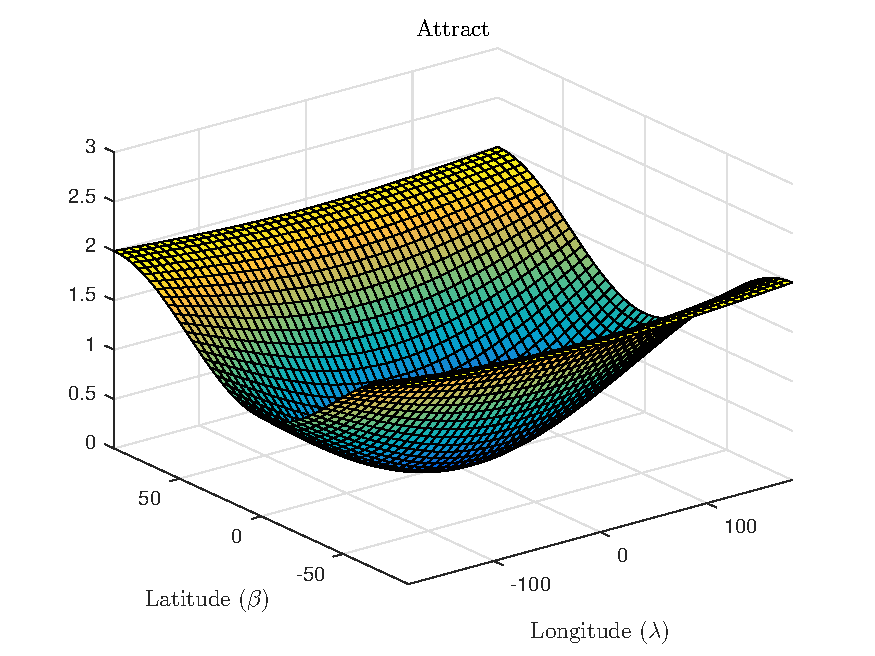
\includegraphics[width=\textwidth]{attract_error}
	\end{subfigure}~
	\begin{subfigure}[b]{0.3\textwidth} 
		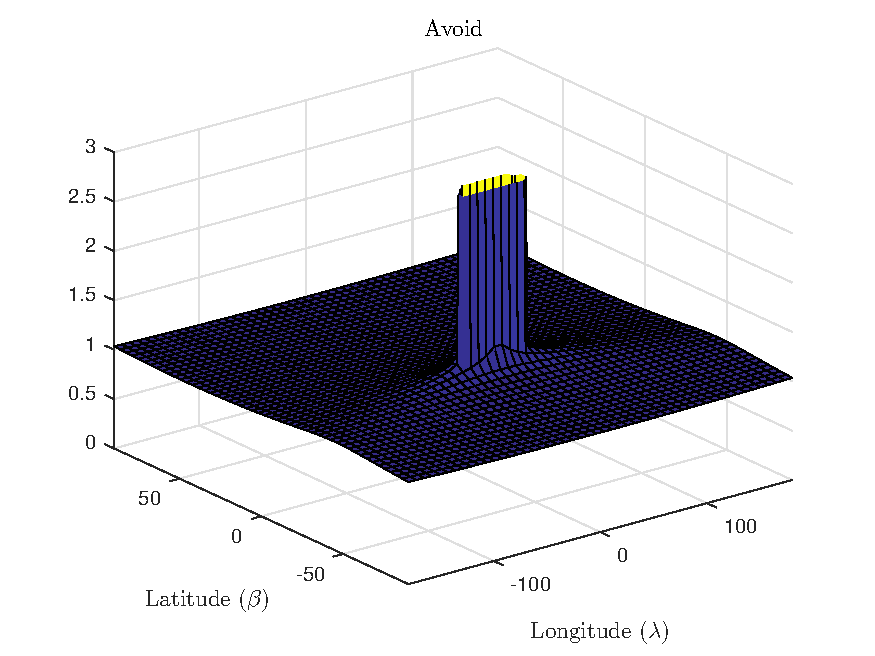
\includegraphics[width=\textwidth]{avoid_error}
	\end{subfigure}~
	\begin{subfigure}[b]{0.3\textwidth} 
		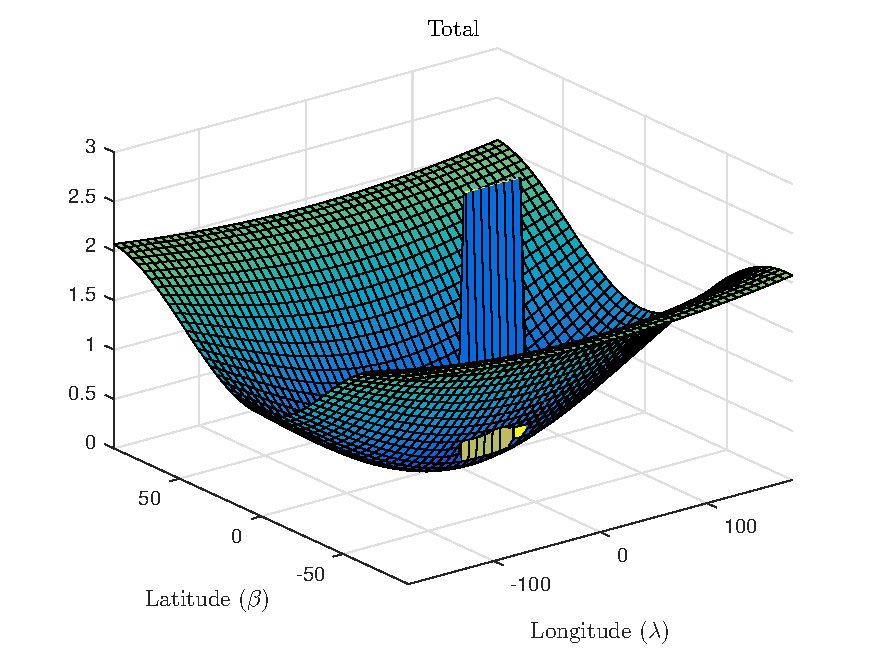
\includegraphics[width=\textwidth]{combined_error}
	\end{subfigure}
\end{figure}
}
\end{frame} %---------------------------------------------------%

\begin{frame}{Controller Design} %--------------------------------------------%
	\begin{block}{Adaptive Attitude Controller}
		Zero equilibrium of error vectors are Lyapunov stable, furthermore \( e_R , e_\Omega \to 0 \) as \( t \to \infty \)
		\begin{align*}
			u &= - k_R e_R - k_{\Omega} e_{\Omega} + \Omega \times J \Omega - W \bar{\Delta} \\
			\dot{\bar{\Delta}} &= k_\Delta W^T \parenth{ e_\Omega + c e_R }
		\end{align*}
	\end{block}
\end{frame}%--------------------------------------------------------------%

\subsection{Simulation results}

\begin{frame}{Simulation} %---------------------------------------------%
\begin{itemize}
	\item Can easily handle multiple constraints
	\item \href{https://youtu.be/dsmAbwQram4?t=20s}{UAV Experiment}
	\item Several benefits over previous methods:
		\begin{itemize}
			\item Avoids attitude parameterizations
			\item Efficient - feedback form
			\item Stability guarantee in spite of disturbances
		\end{itemize}
\end{itemize} 
\animategraphics[autoplay,loop,width=0.45\textwidth]{12}{./animation/sc_avoid_nodist/sc_avoid_nodist-}{0}{99}
\animategraphics[autoplay,loop,width=0.45\textwidth]{12}{./animation/sc_avoid_mult/sc_avoid_mult-}{0}{99}
\end{frame}%--------------------------------------------------%



\end{document}

